\documentclass[UTF8]{ctexart}
\usepackage{amsmath}
\usepackage{amssymb}
\usepackage{graphicx}
\usepackage{geometry}
\usepackage{ctex}
\geometry{a4paper, margin=1in}

\title{QTA2025暑期求职笔试训练营-week2}
\author{}
\date{}

\begin{document}

\maketitle

\section*{笔试题目}

\subsection*{1. 随机数}
小U有一个质地不均匀的硬币, 已知这枚硬币正面朝上的概率$p$不是0或0.5, 但不知道确切的概率, 可以只用这枚硬币帮小U生成100个0~15之间均匀分布的随机整数吗? 小U是个追求严谨的小朋友, 如果可以, 需要聪明的你证明这种策略下生成的随机数的分布严格服从上述要求; 如果不可以, 也请给出证明。

这个问题的核心在于如何利用有篇的随机源来构建概率均等的随机数,我们考虑如下策略,将硬币连续抛掷两次 :
\begin{itemize}
    \item 如果结果是 正-反 (HT),我们就将其记为 0。

    \item 如果结果是 反-正 (TH),我们就将其记为 1。
    
    \item 如果结果是 正-正 (HH) 或 反-反 (TT),我们就舍弃这次结果,重新抛掷两次。    
    
\end{itemize}

\textbf{第一步:验证该策略确实可以生成我们要求的随机数}

设硬币正面朝上的概率为 $p$,反面朝上的概率为 $1-p$(其中 $p \neq 0, 0.5, 1$)。

计算各种情况的概率:
\begin{align}
P(HT) &= p \cdot (1-p) \\
P(TH) &= (1-p) \cdot p = p \cdot (1-p) \\
P(HH) &= p^2 \\
P(TT) &= (1-p)^2
\end{align}

注意到$P(HT) = P(TH) = p(1-p)$

在条件概率下:
\begin{align}
P(\text{输出0} | \text{不拒绝}) &= \frac{P(HT)}{P(HT) + P(TH)} =
\frac{p(1-p)}{2p(1-p)} = \frac{1}{2} \\
P(\text{输出1} | \text{不拒绝}) &= \frac{P(TH)}{P(HT) + P(TH)} =
\frac{p(1-p)}{2p(1-p)} = \frac{1}{2}
\end{align}

因此,每次生成的随机数都是公平的,即 $P(\text{输出0}) = P(\text{输出1}) =
\frac{1}{2}$。

\textbf{第二步:生成0-15的均匀分布}

考虑到是生成16个数,我们可以二进制来处理,具体来说:
\begin{enumerate}
    \item 使用上述方法生成4个概率均等的随机数 $b_3b_2b_1b_0$
    \item 将这上面的随机数转换为整数:$n = 8b_3 + 4b_2 + 2b_1 + b_0$
    \item 由于 $n \in \{0,1,2,\ldots,15\}$,直接输出 $n$
\end{enumerate}

\textbf{证明0-15均匀分布:}

由于每次生成的单个随机数都是独立且公平的($P(b_i = 0) = P(b_i = 1) = \frac{1}{2}$),所以:

$$P(n = k) = P(b_3b_2b_1b_0 \text{的二进制表示为} k) = \left(\frac{1}{2}\right)^4 =
\frac{1}{16}$$

对于所有 $k \in \{0,1,2,\ldots,15\}$ 都成立。

\textbf{生成100个随机数:}

重复上述过程100次,每次生成一个0-15之间的随机整数。由于每次生成都是独立的,且每个整
数的概率都是 $\frac{1}{16}$,所以生成的100个数严格服从0-15的均匀分布。

\textbf{算法复杂性分析:}

每次生成一个公平比特的期望抛硬币次数为:
$$E[\text{抛硬币次数}] = \frac{2}{P(HT) + P(TH)} = \frac{2}{2p(1-p)} =
\frac{1}{p(1-p)}$$

生成4个比特需要期望 $\frac{4}{p(1-p)}$ 次抛硬币。

因此,生成100个0-15的随机整数需要期望 $\frac{400}{p(1-p)}$ 次抛硬币。

\textbf{结论:}

该策略理论上完全可行,生成的随机数严格服从0-15的均匀分布。算法的效率取决于硬币的偏度
 $p(1-p)$,当 $p$ 接近0.5时效率最高。

\subsection*{2. 剪纸转圈圈}
\subsubsection*{(1)}
小U在做剪纸小游戏, 他先剪了一大一小两个圆, 如图1所示, 其中圆A的半径为1, 圆B的半径为5。现在让小圆A绕着大圆B滚动旋转, 请问小圆A旋转多少圈后其圆心将再次到达起点?

\subsubsection*{(2)}
小U又剪了一个边长为1的小正方形C, 现在让小正方形C在大圆B的圆周上移动一周 (保持正方形始终直立, 如图2), 请聪明的你帮小U算一算: 小正方形C平移一周所覆盖区域的面积是多少?

\begin{figure}[h!]
    \centering
    \begin{minipage}{0.45\textwidth}
        \centering
        % The user needs to provide the image file 'figure1.png'
        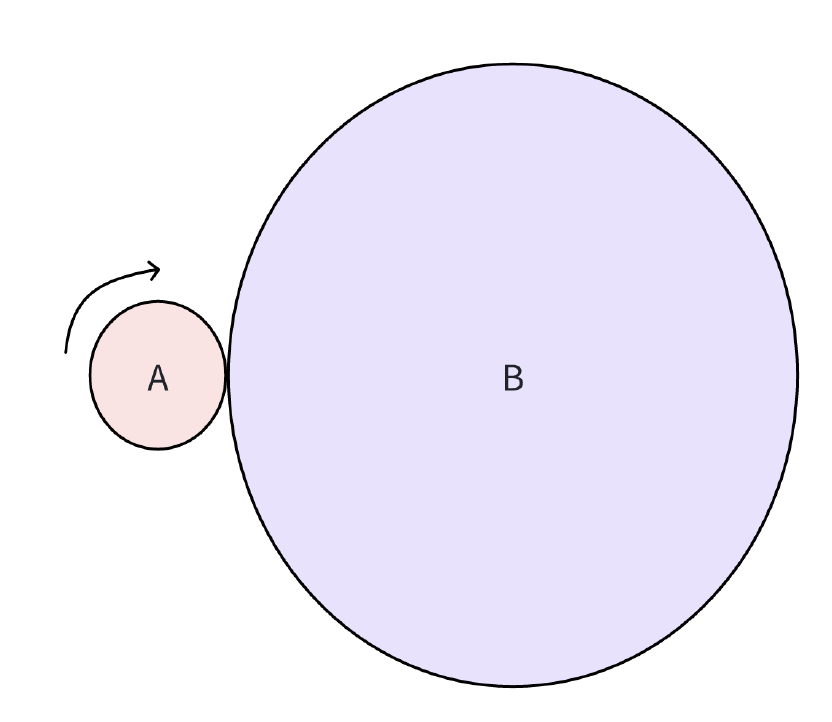
\includegraphics[width=0.8\linewidth]{Figure1.png} 
        \caption{小圆A绕大圆B滚动}
        \label{fig:fig1}
    \end{minipage}\hfill
    \begin{minipage}{0.45\textwidth}
        \centering
        % The user needs to provide the image file 'figure2.png'
        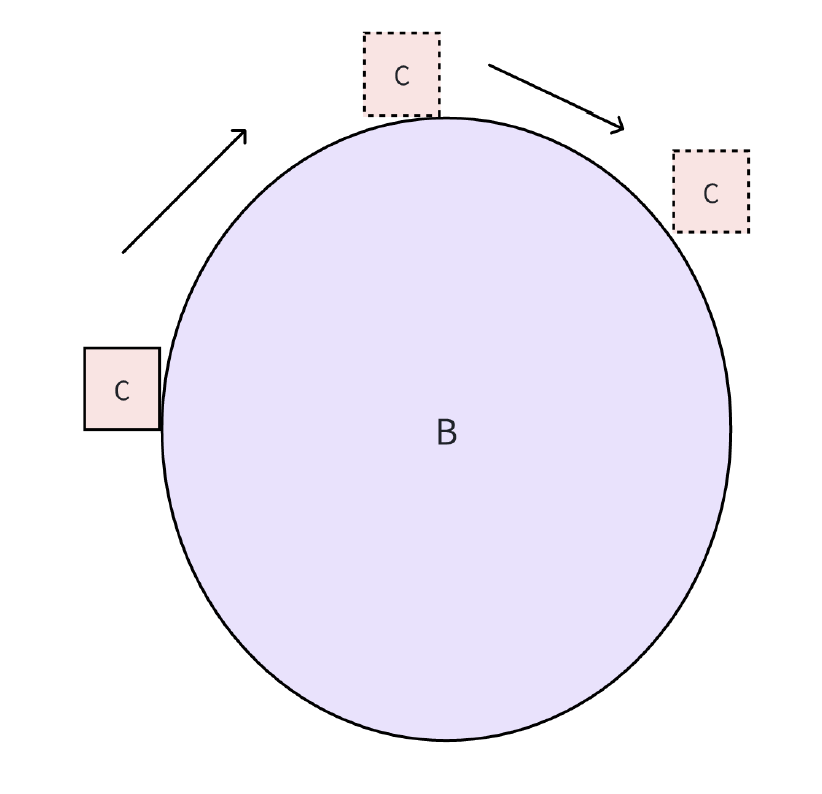
\includegraphics[width=0.8\linewidth]{Figure2.png}
        \caption{正方形C沿大圆B移动}
        \label{fig:fig2}
    \end{minipage}
\end{figure}


\subsection*{3. 正态分布}
概率论和微积分是一个quant需要熟练掌握的基础知识, 小U正在温习正态分布的相关内容。设 $\varphi(y)$ 和 $\Phi(y)$ 分别为标准正态分布的密度和分布函数, 求:
$$
\int_{-\infty}^{+\infty}{\left(y+\frac{1}{\sqrt{\pi}}\right)^{2}(1-\Phi(y))\varphi(y)dy}
$$

\subsection*{4. 打家劫舍}
小U在复习完数学后觉得coding也不能落下, 请聪明的你帮他设计一个时间复杂度尽可能小的算法, 求一个整数数组S中不含相邻元素的子序列的最大和。

\subsection*{5. Linear Regression Model}
Xiao U is learning English and regression analysis. Please help him solve the following problem:
Suppose we have a simple linear regression model,
$$ y_{j}=\beta_{0}+\beta_{1}x_{j}+\epsilon_{j}, \quad j=1,2,...,n $$
But the $x_{j}$ are independently $N(\mu_{x},\sigma_{x}^{2})$. We assume further that $\epsilon_{j}\sim N(0,\sigma_{e}^{2})$, independently of the $x_{j}$'s.
Suppose further that $x_{j}$ is in fact measured with error, so the observations are $(y_{j},w_{j})$, where
$$ w_{j}=x_{j}+u_{j}, \quad u_{j}\sim N(0,\sigma_{u}^{2}) $$
and $u$ is independent of both $x$ and $\epsilon$.
Now, please show that $E(y_{j}|w_{j})=\alpha_{0}+\alpha_{1}w_{j}$, and give expressions for $\alpha_{0}$ and $\alpha_{1}$ as functions of known constants.

\subsection*{6. 共半球问题}
\subsubsection*{(1)}
小U发现了一道经典的量化题: 圆上随机取N个点, 它们在同一个半圆内的概率有多大?

\subsubsection*{(2)}
求知欲很强的小U继续探索, 假如问题变成3维球体呢? 即在球面上随机取N个点, 它们在同一个半球内的概率有多大?

\subsubsection*{(3) 【拓展思考题】}
在n维空间的球面上随机取N个点, 它们在同一个半球内的概率有多大?

\subsection*{7. Pattern Problem}
小U在学习stochastic process, 他手里有一个不均匀的硬币, 每次掷到正面(H)的概率为p, 掷到反面(T)的概率为q, $p+q=1$, 请问首次掷到以下pattern的期望投掷次数为多少?
\begin{enumerate}
    \item HHHHHHTTTTTT
    \item HHHHHHHHHHHH
    \item HTHTHTTHTHT
\end{enumerate}

\end{document}